
\subsection{Shot noise}
\label{sec:shot-noise}

\subsection{Radiation pressure noise}
\label{sec:radi-press-noise}


\subsection{Newtonian Noise}
\label{sec:newtonian-noise}

Newtonian noise, or gravitational gradient noise, is the strain
produced by gravitational coupling between local mass density
variations and the test masses in the interferometer. Examples of
significant sources of Newtonian noise include clouds passing overhead
the detector, and seismic perturbations in the local ground density.

\subsection{Seismic, Newtonian, and thermal noise}
\label{sec:seismic-noise}

Seismic noise is the result of strain introduced into the
interferometer through movement of the ground, which can be the result
of geophysical activity, tidal activity, or anthropogenic sources of
seismic noise, such as road traffic or railways. Seismic noise is also
a source of Newtonian noise (see section \ref{sec:newtonian-noise})
due to density fluctuations as the seismic wave passes through the
ground.
\sidebar{
  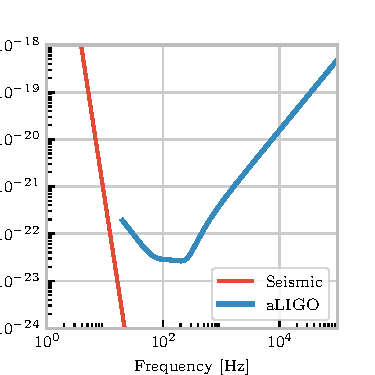
\includegraphics{figures/seismicnoise-psd.pdf}
  \captionof{figure}{The seismic noise power spectral density for a ground-based interferometer, compared to the PSD for Advanced LIGO at its design sensitivity.}
  }
One of the important considerations in choosing a site for an
interferometer is the presence of seismic noise, and for this reason
they are normally located far from urban areas. Despite this, both of
the Advanced LIGO sites are affected by the presence of loud
anthropogenic noise sources (LHO is affected by a nearby Department of
Energy site; LLO is affected by logging activity and a nearby railway
track)\cite{2004CQGra..21.2255D}. LLO is also strongly affected by
severe storms due to its proximity to the Gulf of Mexico.

\begin{table}
  \begin{tabular}{ccl}
    \toprule
    $f$ [Hz] & $D$ [km] & Sources \\
    \midrule
    0.01--1.0    &  1000         & Earthquakes, microseism \\
    1--3 & 10 & Anthropogenic, nearby earthquakes, wind \\
    3--10 & 1 & Anthropogenic, wind \\
    10--100 & 0.1 & Nearby Anthropogenic noise\\
    \bottomrule
  \end{tabular}
  \caption{The principle seismic noise frequency bands which affect ground-based detectors, their sources, and the distance over which the band affects advanced-generation detectors.}
  \label{tab:seismic-bands}
\end{table}
}

Seismic noise limits the sensitivity of the second generation
detectors at low frequencies ($f < \SI{50}{\hertz}$), but it is
present as a noise source across the passband of the detector. The
seismic noise shows a pair of notable peaks below the $\SI{1}{\hertz}$
level, one caused by ocean swell, which has a period around 4 to 30
seconds, and a second caused by standing seismic modes in the Earth
which spans the range of 30 to 1000 seconds. The presence of seismic
noise below $\SI{30}{\hertz}$ is still problematic for ground-based
interferometers, depsite this being outside the design frequency
range, due to \emph{upconversion}, where low-frequency noise couples
non-linearly into higher frequency noise.

Coupling of seismic noise into a detector's Differential Arm Length
Displacement read-out (DARM) is given by
\begin{equation}
  \label{eq:darm-seismic}
  L(f) = 2 \frac{N_{\rm grav}(f)}{(2 \pi f)^2}, \quad N_{\rm grav}(f) =  \beta G \rho  N_{\rm sei}(f)
  \end{equation}
  for $N_{\rm grav}$ the fluctuation of the local gravitational field
  projected onto the axis of the arm cavity, $\rho$ is the ground
  density near the test mass, $\beta \sim 10$ is a geometrical factor,
  and $N_{\rm sei}$ is the seismic motion near the test
  mass\cite{2016PhRvD..93k2004M}.

Seismic isolation is used in detectors to reduce the noise level due
to seismic activity. This takes two forms: active isolation, and
passive isolation. The former is accomplished by mounting optical
components on hydraulic external pre-isolator (HEPI) systems which are
controlled, via a feed-forward system, to a seismometer. The latter is
reduced by suspending the optics as a component in a pendulum
system. In the Advanced LIGO design this involves the test masses and
their associated mirrors composing the final component in a quadruple
pendulum suspension.

\sidebar{
  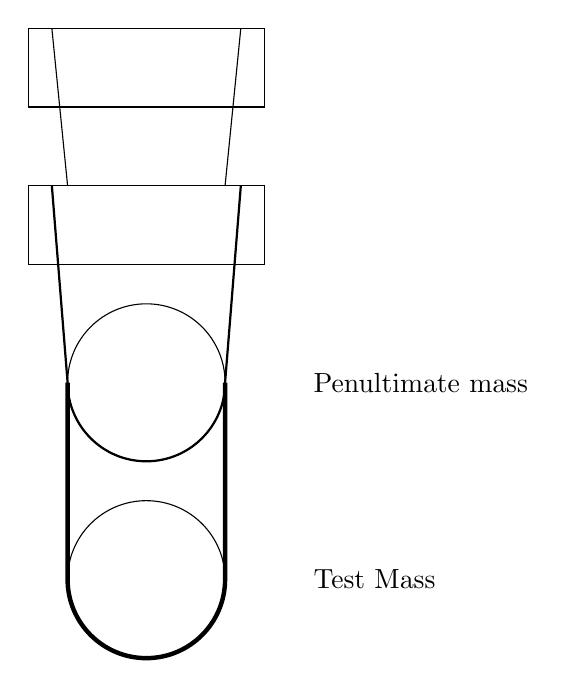
\begin{tikzpicture}[]
	\draw (0,0) circle (1) node [right = 2cm] {Test Mass};
	\draw (0,2.5) circle(1) node [right=2cm] {Penultimate mass}; 
	\draw (-1.5,5) rectangle (1.5,4);
	\draw (-1.5,7) rectangle (1.5,6);
	\draw [thick] (-1.2,5) -- (-1, 2.5)  arc (180:270:1)-- (0, 1.5) arc(90:180:-1) -- (1.2,5);	
	\draw [ultra thick] (-1, 2.5) -- (-1, 0) arc (180:270:1) arc (90:180:-1) -- (1,2.5);
	\draw (-1.2, 7) -- (-1, 5) (1,5) -- (1.2,7);
      \end{tikzpicture}
      \captionof{figure}{A schematic of the Advanced LIGO quadruple
        suspension; the upper stages are composed of maraging steel,
        and isolate vertical motion from the pendulum; the lower
        stages are silica glass masses. The bottom two stages are
        joined with monolithic silica fibres. \label{fig:quad-susp}}
  }

  In addition to seismic noise other phenomena may cause a change in
  the local gravitational field which will couple into DARM; these noise sources are normally grouped-together as ``Newtonian noise'', and can include the effect 
  
\subsection{Other noise sources}
\label{sec:other-noise-sources}
There are numerous additional noise sources within the interferometer.

%%% Local Variables: 
%%% mode: latex
%%% TeX-master: "../../document"
%%% End: 
